%!TEX root=../tax-democracy-held.tex

%add comment, footnote: this was first submitted as \ldots

%``analytic muddle of tax'' (\citealt{McCaffery2005}: 862)

\begin{quote}
	\emph{``Things in tax are bad today.''}
	\\*
	%better quote
	--- Edward J.\ \citet[893]{McCaffery2005}
\end{quote}

%McCaffery:
	%There are four particularly important ones in tax: the taxable unit, the tax base, the rate structure, and the timing of tax.
%Who pays tax? On what? How much? When? TheseRead more at location 137   • Delete this highlight
	%Note: add this to my systematic Edit

 \begin{figure}[htbp]
	\centering
	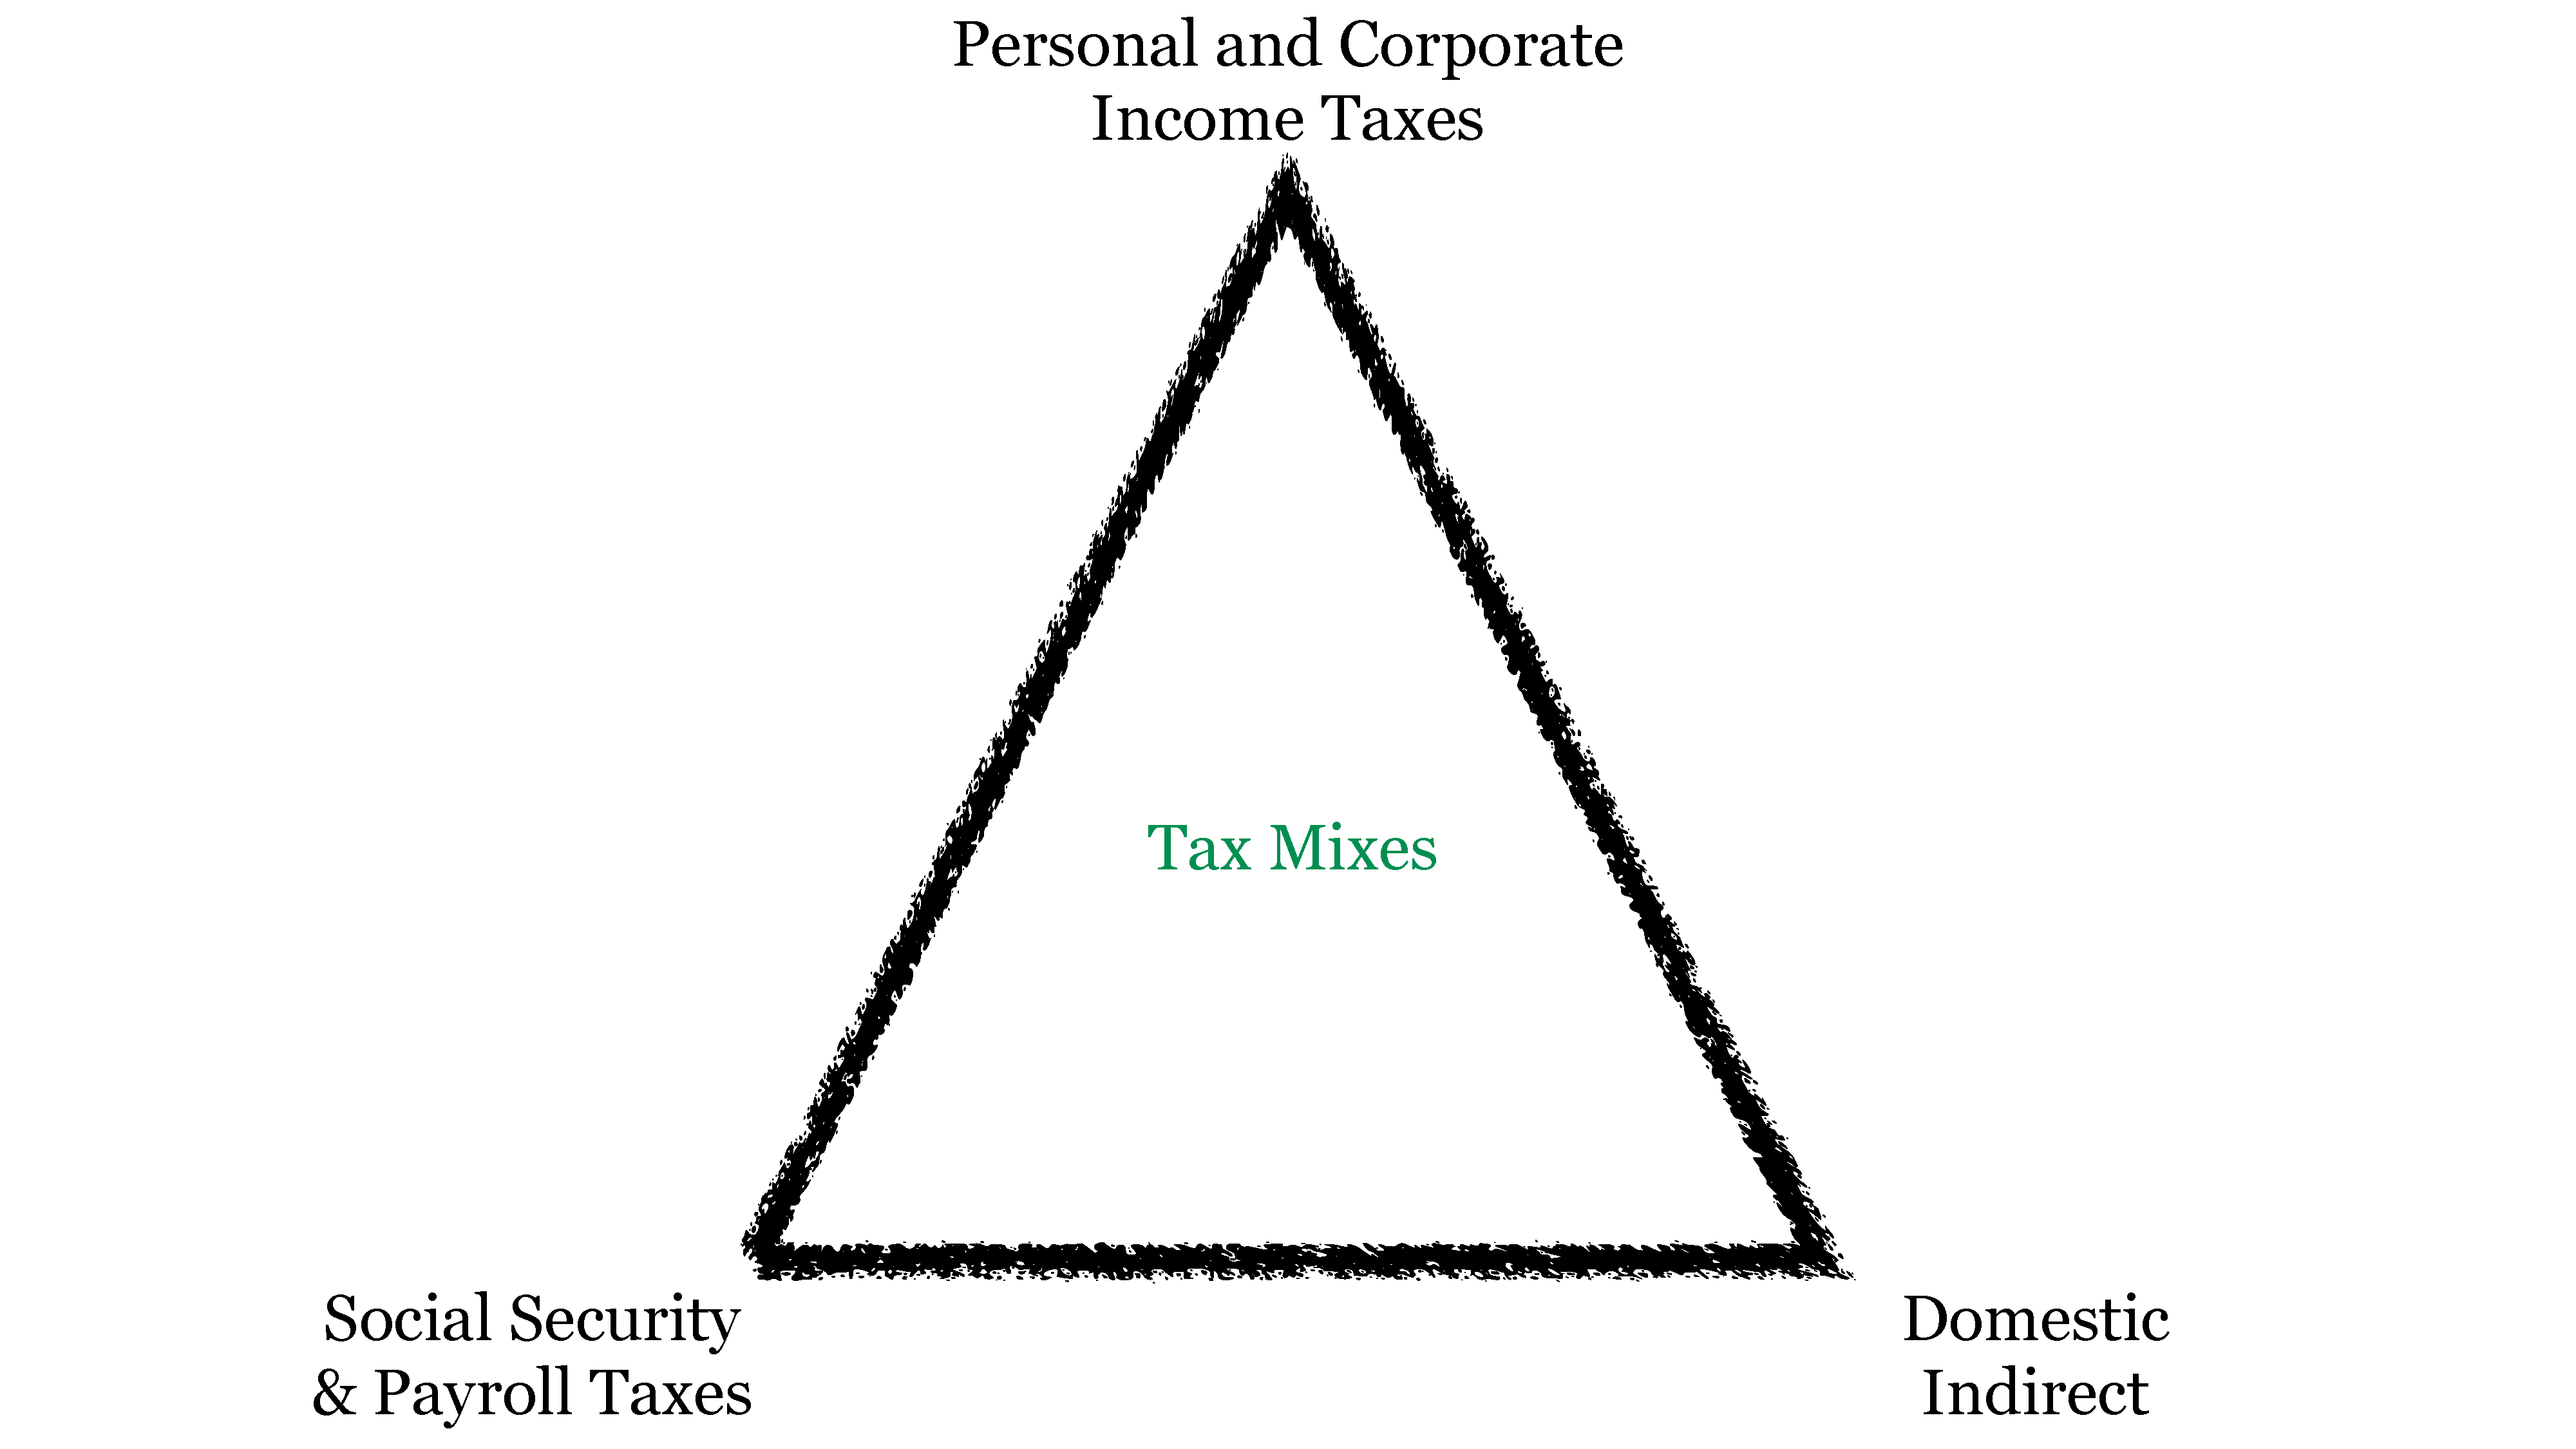
\includegraphics[width=1\linewidth]{tax-mixes}
	\caption[Tax Mixes]{Tax Mixes of Real Existing Welfare States}
	\label{fig:tax-mixes}
	%somehow link this to the other tax
\end{figure}

%here used to be tax-with-trends, it's now in testing-hypotheticals

Designing \hyperref[sec:axiology]{desirable taxation} in the real world is hard.
Economic and administrative complications beset taxation and easily effect undesirable, unintended consequences \citep{Merton-1968-aa}.
Economic complications arise where market participants interact with tax policies.
Administrative complications arise where transactions become complex, or where axiomatically assumed \hyperref[sec:work-play]{distinctions do not hold} in real life (page \pageref{sec:work-play}).
	%circular wording

\section[Incidence]{Incidence:~Doable Taxes Exert Well-Defined Burdens} \label{sec:tax-incidence}
%old title: {\emph{Whom} to Taxed? ---\\Redistributive Taxation is Personal}

%taxing corporations is stupid: they are, and for good reasons, only virtual entities \cite{Coase1937}
	%actually Coase suggests we shouldn't get into this, we should not favor some ways of organizing cooperation over others \ldots

%remind people here about natural persons, but that is in fairness.

%taxes should always be in real terms, never in nomal terms.
%That's studpid otherwise.

Corporate bodies have rightfully been characterized as fictions.
	%source
 The welfare of all these non-natural, private juristic persons ultimately accrues to natural persons as their owners, workers or consumers\footnote{
	Foundations with their earmarked, tax-exempt and free-roaming capital may be a exception to this generalization.
The beneficiaries of a foundation's mission may substitute as natural persons to which the foundations welfare --- albeit involuntarily --- accrues.\\A \href{http://maxheld.de/2010/03/27/foundations-may-be-bad/}{critical acclaim} of the political economy, democratic legitimacy and taxation of supposedly benevolent foundations is direly needed but clearly beyond the scope of this thesis.}.
Equity considerations do not apply at the corporate level\footnote{
	Corporate bodies are, of course, \emph{operative} fictions in their consumption of \href{sec:common-good}{Common Goods} and \href{sec:natural-monopoly}{Natural Monopolies}.
To receive correct price signals, corporate bodies should therefore be subjected to Pigouvian taxes and fees.}.

As per desideratum \ref{des:redistribution-and-revenue-are-one}, \hyperref[des:redistribution-and-revenue-are-one]{redistributive and revenue generating taxes are one}. \ref{sec:fiscal-redistribution-and-revenue-are-one} \ref{des:redistribution-and-revenue-are-one}
It follows that for both these components:

\begin{desideratum}[Personal Taxation]
	A doable tax falls only on natural persons.
	\label{des:personal-taxation}
\end{desideratum}

\paragraph{Love and Marriage}
	\phantomsection
	\label{sec:love-marriage}

\begin{verse}
	\emph{``Love and marriage, love and marriage\\
	Go together like horse and carriage\\
	(\ldots)\\
	Try, try, try to separate them:\\
	It's an illusion.''}\\*
	--- Frank Sinatra (1915-1998)
\end{verse}

%add triangle of impossibility here
Personal taxation becomes impossible when common usage, transfers and mutual obligations become so intensive, informal and intangible as to render individual accounts meaningless.
In modern, functionally differentiated societies such \emph{mechanical solidarity} is --- for better or for worse --- largely replaced by extensive, formalized and tangible \emph{organic solidarity} \citep{Durkheim-1893-aa}.

%for a more comprehensive discussion of gender and tax, especially its interatcion through class, see \cite{McCaffery2009a}
	%also note that imputed income would provide a partial fix for the problem as in \cite[6304]{McCaffery2009a}

Romantic cohabitation, marriage and the nuclear family alone remain as refuges of mechanical solidarity.
Personal taxation of (married) couples and families becomes impracticable.
They are therefore taxed as \emph{one} entity, or at least under one rate.
%does not exist
	%Under \href{des:SharpProgression}{progression} as per desideratum \ref{des:SharpProgression},
A problem arises:
you have to add (two) potentially (very) different incomes\footnote{The problem occurs in equivalent form when a different base for progressive taxation is chosen, for example property or consumption.} together and tax them under a \emph{single} rate.
There are two ways to do this.
First, you can apply the same schedule as for single households, which would punish people just for getting married or having children.
For example, two people earning \$50,000 each would, after marriage, be taxed under the higher rate applicable at \$100,000.
Secondly, you can divide the family income by the number of people in the household and apply the tax rate for this \emph{average} income.
In this case, the tax liability will depend on the \emph{distribution} of incomes \emph{between} the family members.
If their incomes are starkly different, they will benefit from applying a progressive rate to their \emph{average} income.
This conundrum cannot be resolved:
it is the equivalent to \citeauthor{Arrow1950}'s \emph{Impossibility Theorem} in taxation.
Of three desirable things, you can only have two:
\begin{enumerate}
	\item \href{des:SharpProgression}{a progressive schedule},
	\item neutrality towards marriage and
	\item tax liability independent of the distribution of income in a household (\citealt[124]{Moffitt2003}, \citealt[29]{Dalsgaard2005})
\end{enumerate}
.
	%add: practical: anything inbetween, but still same problem

I have stated here that progression is desirable, and that people should not and cannot be punished for mechanical solidarity in family and marriage.
% \href{des:SharpProgression}{progression}
It follows that, while undesirable, the tax liability \emph{will} be dependent on the distribution of income in a household.

The contradictions arising in the taxation of family and marriage point to more fundamental \href{sec:work-play}{problems of drawing boundaries} (page \pageref{sec:work-play}) based on administrative and analytical abstractions (here:
\hyperref[des:personal-taxation]{taxation of natural persons}, page \pageref{des:personal-taxation}) that are not unambiguously applicable in real life.
As this particular problem affects all progressive taxes, it will not be further addressed here.

 The aggregate costs of taxation depend on the responsiveness, or elasticities of what is being taxed.
The individual costs --- who \emph{really} pays --- also depend on this responsiveness.

\paragraph{Flypaper Theory is False.}
To illustrate this dynamic, first consider \autoref{fig:same-incidence}.
In this market (actually the same as in \autoref{fig:DWL}), a tax is placed on the supplier.
For any given market price, the producer is now willing to produce less.
The supply curve shifts upwards by exactly the amount of the tax.
Assuming constant demand, the curtailed supply will raise the price above the prior equilibrium.
Both consumers and producers end up paying for the tax.
Consumers have to buy at higher prices.
Producers have to sell at lower prices.
In this case, consumers and producers carry an equal share of the tax burden.
\footnote{
	In this illustration, the costs to consumers and producers are only the product of the post-tax quantity and the prices they receive, respectively.
	In \autoref{fig:DWL} these are the rectangles $B$ and $C$ formed by the price difference to equilibrium prices at post-tax quantities.
	An equivalent mechanism operates to distribute the burden of the DWL, or the foregone consumption (production) at lower (higher) prices.
	The DWL is also split evenly between consumers and producers in this case.
	More generally, the DWL is split according to relative elasticities of supply and demand:
	whichever is less elastic, bears the greater DWL.
	The ``incidence'' of DWLs is customarily not included in assessments of tax incidence, precisely because tax incidence is concerned with the ultimate origin of tax \emph{revenue}.
	The DWL, by definition, is that welfare lost that is \emph{not} recouped as tax revenue.
}
%this figure is already in mixed economy.
%It's now fig:same-incidence

The naive ``flypaper theory of tax incidence'' is false:
the state cannot easily legislate \href{sec:fiscal-redistributionIsPersonal}{who \emph{should} pay} a tax.
Instead it must anticipate market reactions to the tax and gauge the \emph{effective} incidence, irrespective of where the tax was originally levied.
\footnote{
	The usual assumption is that incidence applies only to indirect taxes (VAT, Corporate Income Tax).
	I find this limited application of incidence implausible.
	The concept remains applicable for direct taxes (Personal Income Tax (PIT), Asset Tax), too.
	A PIT on labor incomes, for instance, may partially fall on employers when labor markets are very tight:
	tax-depressed worker supply may lead employers to pay more.
	Even an Asset Tax may fall on people other than the owners when demand for their collateral is sufficiently inelastic:
	interest rates may rise when private capital becomes less abundant.
	A more complete discussion of the incidence of the different taxes must await \autoref{sec:contest} on page \pageref{sec:contest}.
}
		%really? Asset Tax?

\paragraph{The Relatively Less Elastic Bears Relatively More.}
The incidence is not only different from where a tax is levied, it can also fall asymmetrically on demand and supply.
More specifically, the incidence of a tax is determined by the \emph{relative} price elasticities of supply and demand:
whoever is less elastic (more inelastic) bears a relatively greater share of the burden.

\autoref{fig:different-incidence} illustrates the incidence of a tax on suppliers in a market with relatively less elastic (more inelastic) demand.
It is the same market as in \autoref{fig:same-incidence} and \ref{fig:DWL}, only the elasticity of demand is different:
buyers react relatively less to price changes than sellers.
As a result, buyers are willing to pay quite a lot to maintain a similar quantity.
Sellers, by contrast, will curtail their production substantially when prices drop.
The market reaches a post-tax equilibrium at a price much greater than pre-tax equilibrium for consumers, and a little lower for producers.
Consumers end up bearing most of the burden.

%this figure is now in mixed economy.
%fig:different-incidence

%generally, make a big overview of different taxes and taxonomy used here just to make it easier for people to follow.
%Put it in the appendix.

\paragraph{Incidence is Hard.}
As argued in the above, relative price elasticities of demand and supply can be hard to ascertain ex-ante, and they are affected by many factors.
To reliably gauge the effective incidence of a tax, government would have to know the elasticities in a myriad of markets and constellations with great precision.
This will be very costly and likely unsuccessful.
	%does the PCT really have a good incidence? Think mercedes/daimler


To effectively redistribute between \href{des:personal-taxation}{natural persons only}, as per desideratum \ref{des:personal-taxation}, a doable tax will fall on market interactions where relative elasticities of demand and supply can be easily and reliably ascertained.
Government can achieve non-random, normatively justifiable redistribution only when:

\begin{desideratum}[Determined Incidence]
	A doable tax has a well-determined incidence.
	\label{des:determined-incidence}
\end{desideratum}

\section[Elasticity]{Elasticity:~Doable Taxes Hardly Alter Economic Exchanges}
	\label{sec:tax-elasticity}
	%{\emph{How} to Tax? ---\\Taxing Inelastic Bases Minimizes DWLs} \label{sec:tax-elasticity}
Desideratum \ref{des:minimal-DWL} holds that \href{des:minimal-DWL}{a desirable tax should have a minimal deadweight loss}.
A DWL arises when the tax revenue recouped is smaller than the consumer and producer surplus lost as a result of depressed market exchanges or gains from trade (see \autoref{fig:DWL}).
A doable tax with a minimal DWL will fall on market exchanges that respond little to the resulting price change.

\paragraph{Responsiveness is Elasticity.}
This responsiveness is called the \emph{price elasticity} of demand and supply respectively.
It is defined as the percent change in quantity demanded (supplied) over a percent change in price \citep{Marshall1890}.
Where $E-{d}$ ($E-{s}$)  is the price elasticity of demand (supply), $Q-{d}$ ($Q-{s}$) the quantity demanded (supplied) and $P$ the price, it holds that:

	\begin{equation} \label{eq:PED}
			E-{d}=\frac{\%\ \mbox{change in quantity demanded}}{\%\ \mbox{change in price}}=\frac{\Delta Q-{d}/{Q-{d}}}{{\Delta P}/{P}}
	\end{equation}

 and

 	\begin{equation} \label{eq:PES}
			E-{s}=\frac{\%\ \mbox{change in quantity supplied}}{\%\ \mbox{change in price}}=\frac{\Delta Q-{s}/{Q-{s}}}{{\Delta P}/{P}}
	\end{equation}.

\paragraph{Elasticities of Supply and Demand}
become more intuitive when applied in polar cases of \href{fig:inelastic}{perfect inelasticity} (\autoref{fig:inelastic}) and \href{fig:elastic}{perfect elasticity} (\autoref{fig:elastic}).

%I definetely NEED to look into the Harbinger triangle literature on the costs of taxation.
%This seems to be different from this (Marshallian?) view based on consumer surplus.
%There's also a view based on (Pigou?), asking whether the loosers (the taxpayers) can be compensated by the winners (the recipients of subsidies).

\subparagraph{Perfectly elastic}
supply (demand) does not respond at all to changes in price.
Whatever the price, suppliers (buyers) will always produce (buy) the same quantity.
It is displayed by a perpendicular supply (demand) curve in \autoref{fig:inelastic}.

\subparagraph{Perfectly inelastic}
supply (demand) responds maximally to minimal changes in price.
When the price drops (rises) below a certain point, suppliers (buyers) will cease stop producing (buying) any quantity.
Below (above) the horizontal supply (demand) curve in \autoref{fig:elastic}, no production (buying) occurs at all.

 \begin{figure}[htbp]
	\centering
	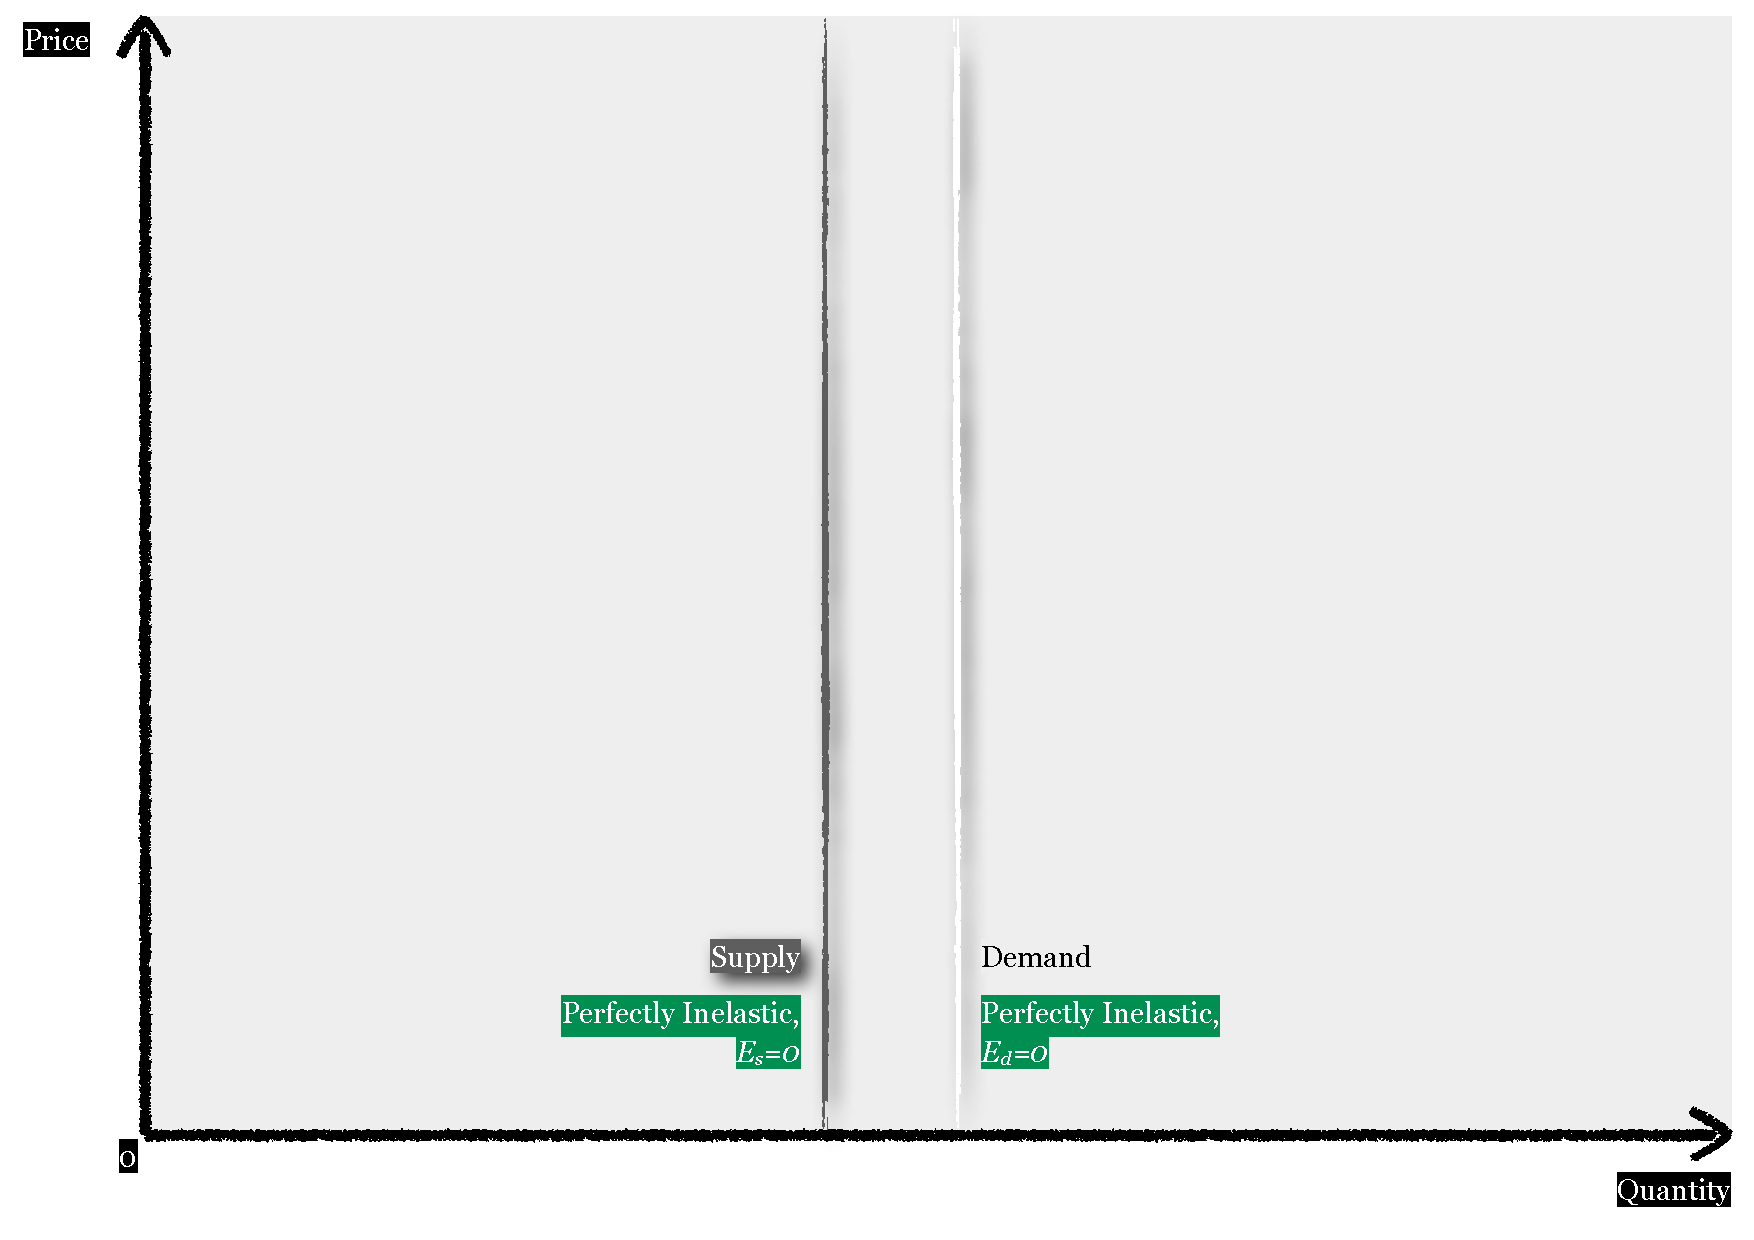
\includegraphics[width=1\textwidth]{inelastic}
	\caption{Perfectly Inelastic Supply and Demand}
	\label{fig:inelastic}
\end{figure}

 \begin{figure}[htbp]
	\centering
	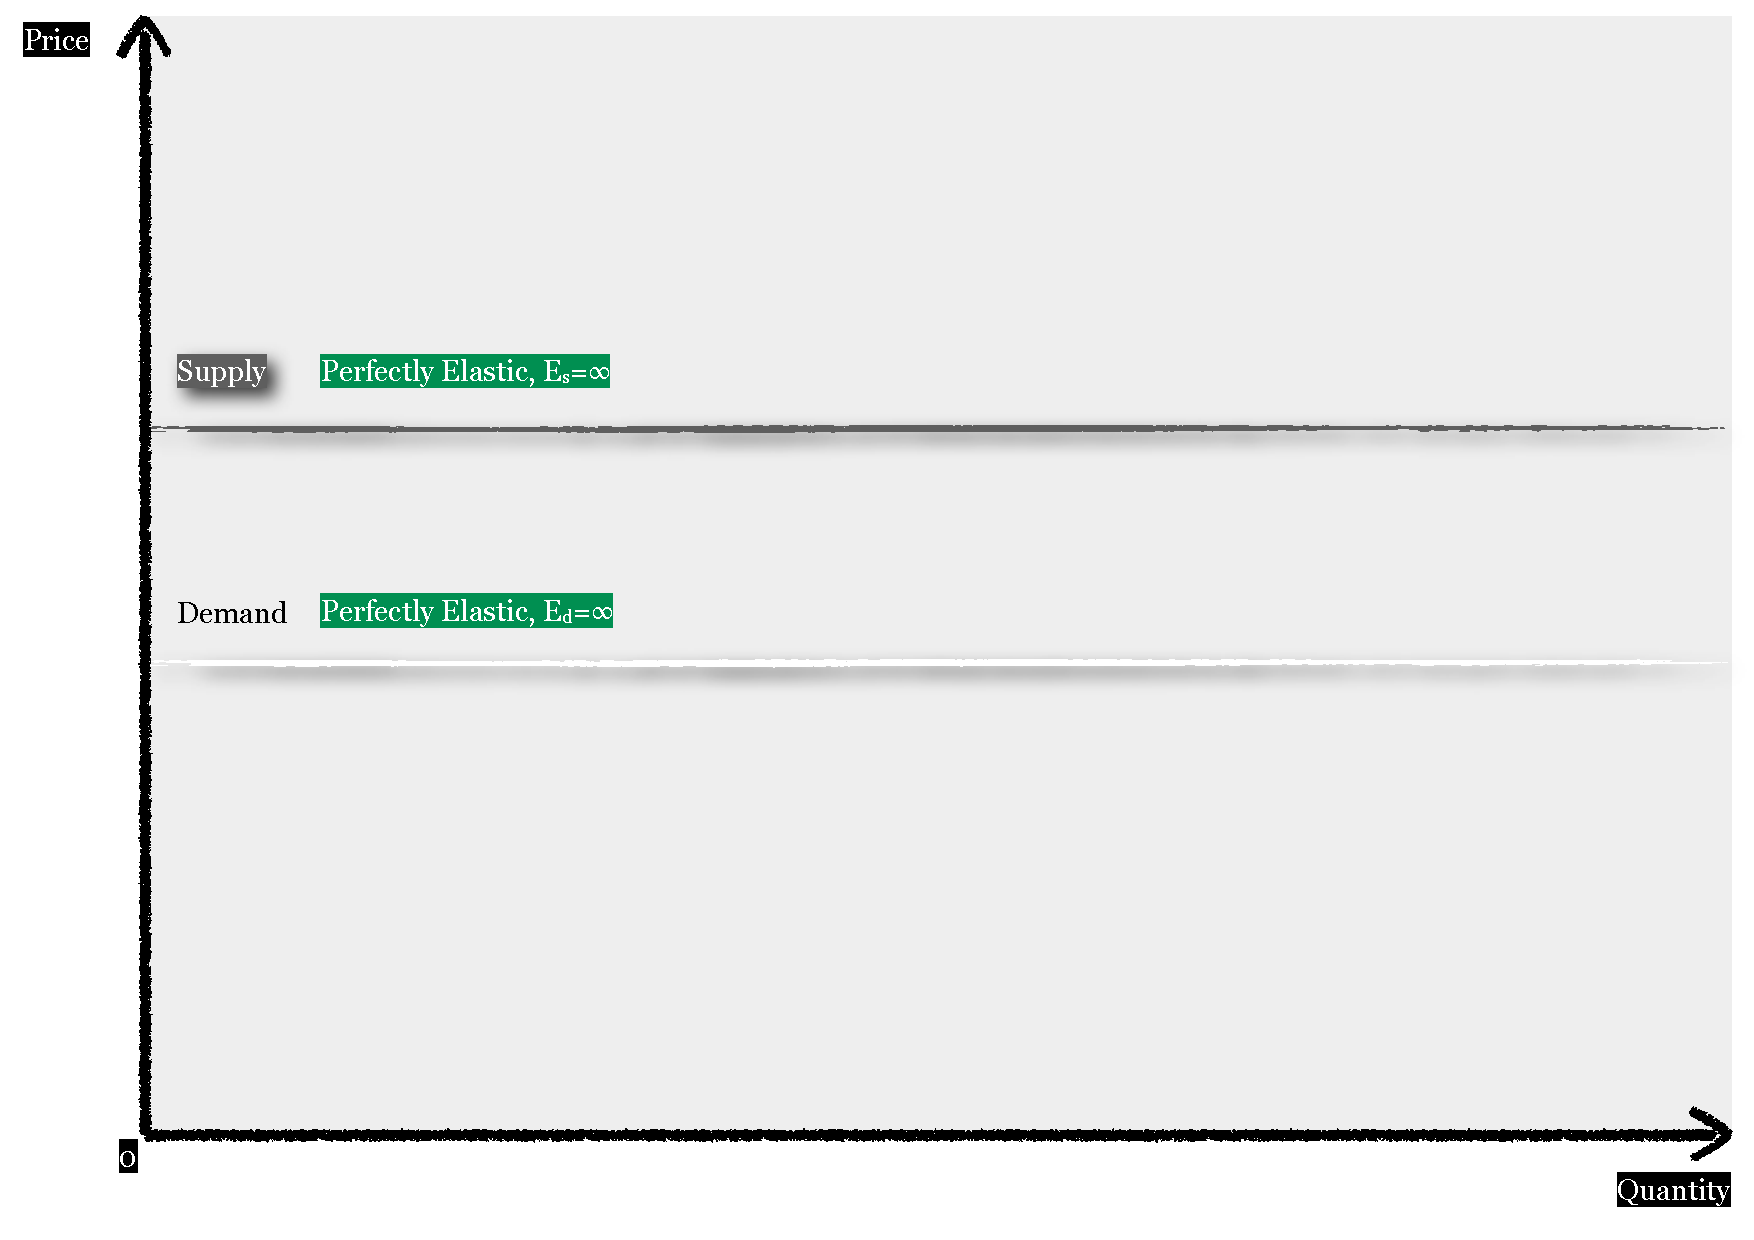
\includegraphics[width=1\textwidth]{elastic}
	\caption{Perfectly Elastic Supply and Demand}
	\label{fig:elastic}
\end{figure}

 \begin{figure}[htbp]
	\centering
	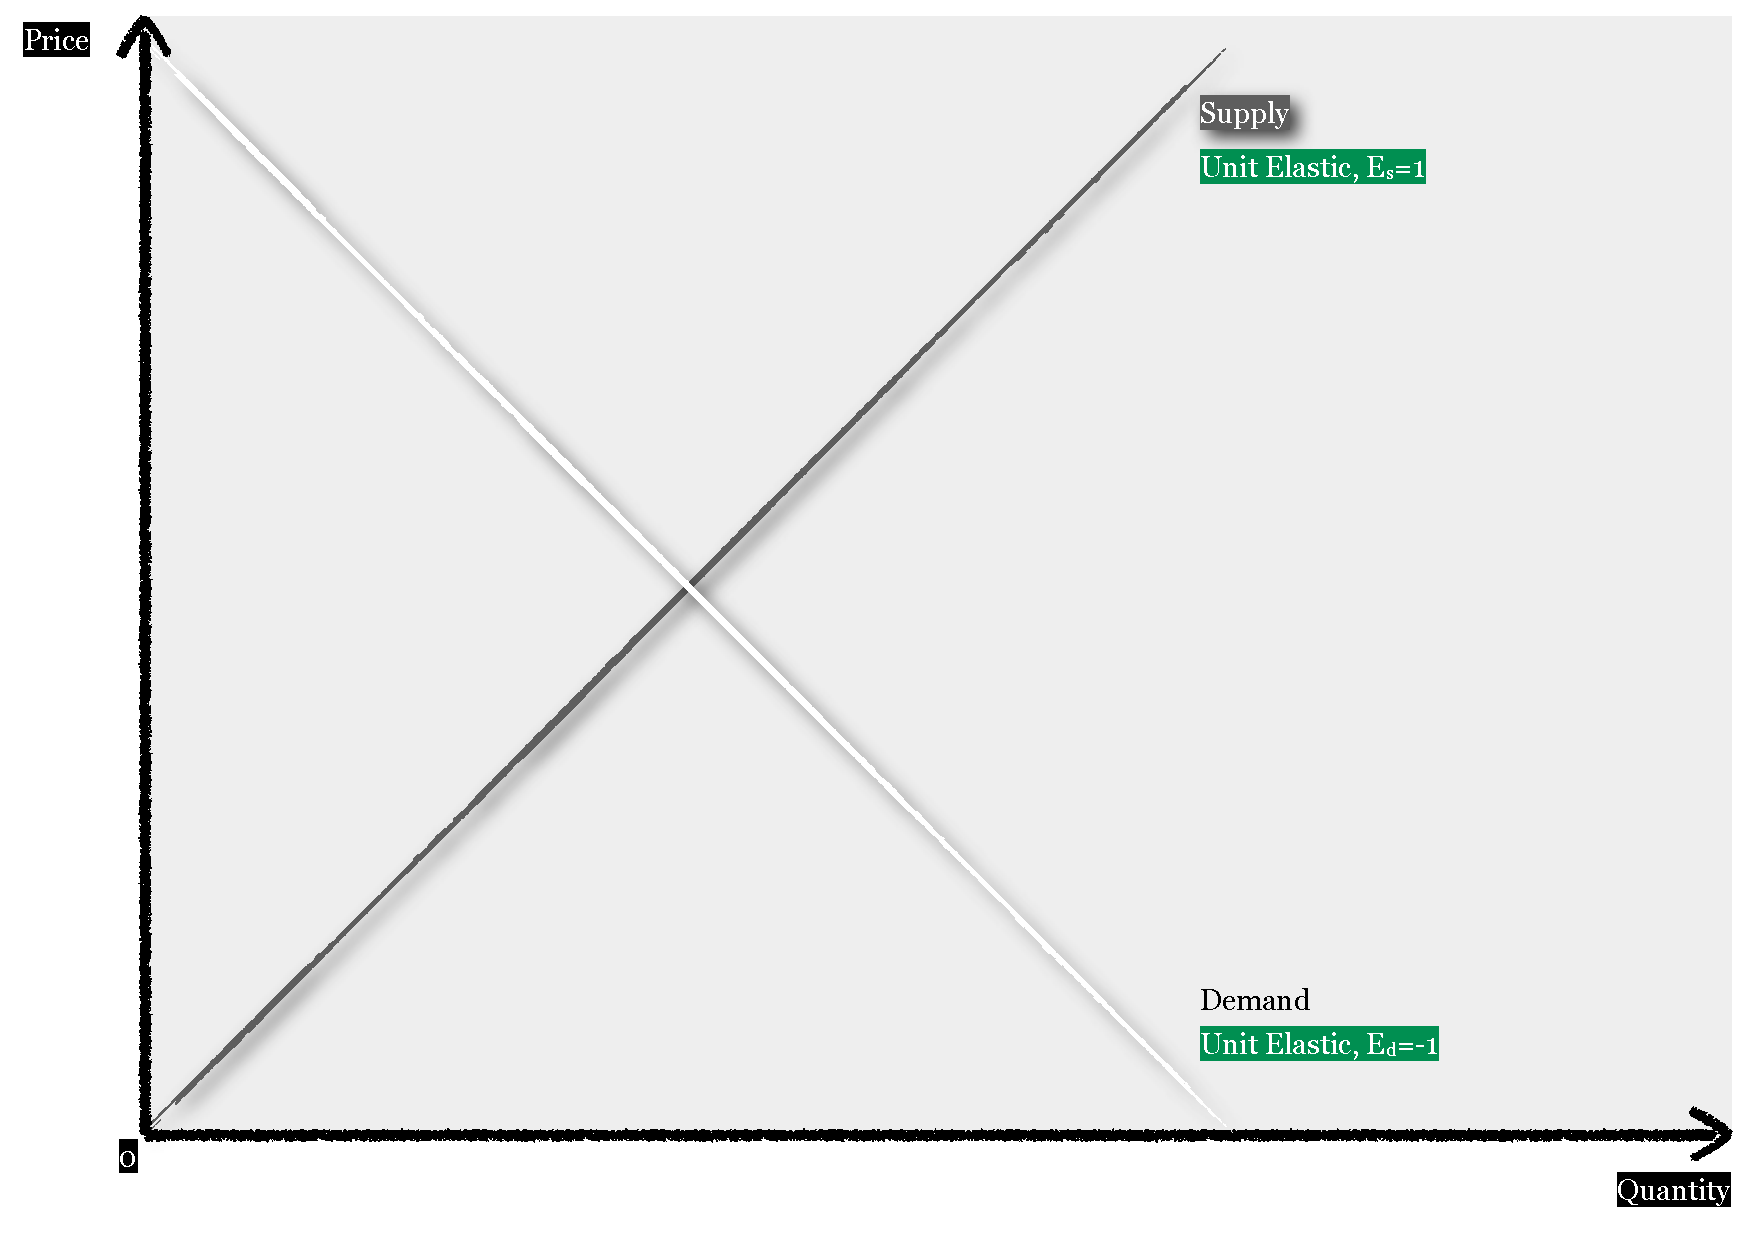
\includegraphics[width=1\textwidth]{unit-elastic}
	\caption{Unit Elastic Supply and Demand}
	\label{fig:unit-elastic}
\end{figure}

\subparagraph{Unit elastic}
supply (demand) responds proportionally to changes in price.
Along a supply (demand) curve of slope $1$ ($-1$), producers (buyers) produce (buy) one percent more quantity for each percent increase (decrease) in price\footnote{The complications of point-vs.-arc elasticities are of no relevance here.
For a review, see \cite{Allen1933} and recently, \cite{Vaughan1988}.}.

\paragraph{Elasticities and DWLs.}
Because DWLs stem from market participants tax-depressed activity, less price responsive activities will be more efficient to tax.
Relatively inelastic supply and demand will have relatively smaller DWLs (\citealt{Ramsey}, \citealt[16]{Piatkowski2008}).

%this figure is now in mixed economy \label{fig:smaller-DWL}

This is illustrated in figures \ref{fig:DWL} and \ref{fig:smaller-DWL}.
\autoref{fig:smaller-DWL} displays the same market with the same tax, only with relatively less elastic (= more inelastic) supply and demand.
Compared to the original DWL-scenario in \autoref{fig:DWL}, the DWL in \autoref{fig:smaller-DWL} is absolutely smaller and smaller relative to the recouped tax revenue.
Because both producers and buyers are less responsive to the tax-induced price change, they each loose less of their surplus.

A doable specification of desideratum \ref{des:minimal-DWL} on \href{des:minimal-DWL}{minimal DWLs} is:

\begin{desideratum}[Tax Inelastic Bases]
	A doable tax falls on inelastic bases.
	\label{des:tax-inelastic}
\end{desideratum}

\paragraph{Determinants of Elasticity.}
Elasticities are hard to quantify:
if prices change, they typically change only marginally.
Elasticities are typically known only \emph{locally}, that is, in the vicinity of equilibrium prices.

Elasticities are determined by a host of factors.
The price elasticity of supply depends, amongst other things, on the mobility of labor and capital employed in production, the availability of substitute consumers or the ability to substitute current for future sales (a.k.a.
liquidity).
The price elasticity of demand depends, amongt other things, on the availability of substitute goods, brand loyalty or ability to substitute current for future consumption.

\section[Schedule]{Schedule}
	\label{sec:tax-schedule}
%cold progression
%make it smooth, just what must the curve be?
%the first derivative must never be \ldots

%maybe mention here the boundaries on which taxation depends?

\section[Timing]{Timing:~A Doable Tax Falls on Liquid Goods}
	\label{sec:tax-timing} %worry: is this maybe yet another subset of a DWL problem?
%old title: when to tax: measuring economic flows is non-trivial

\subsection{Savings norms}

%does this belong here?
%include here the visualization from McCaffery, note that it is an application of Modigiliani's Life Cycle Income Hypothesis (Wikipedia) (original source is unclear)

\subsection{Liquidity}

%get quote

% via wikipedia on LVT, here's a reason for why govntm evaluation is always bad: Austrian School economist Murray Rothbard later raised similar concerns, stating that no government can fairly assess value, which can only be determined by a free market.[20]
	%Rothbard, Murray.
%"The Single Tax: Economic and Moral Implications and A Reply to Georgist Criticisms".
%The Mises Institute.
%Retrieved 2009-02-13.

Any non-flat distributive norm of taxation requires that \emph{ability to pay} (or some other criterion) is measurable.
  In a non-static economy, this ability will change over time.
It is hard to know exactly \emph{when} welfare accrues to people and can be even harder to measure.

\paragraph{The Good:~Exchanges.}
In perfect, liquid markets exchanges are so frequent, intensive and transparent that the equilibrium valuation of  buyers and sellers can be known at every time and with great precision.
Stock exchanges are a good example:
company stocks are bought an sold so often, by so many people, and so publicly that at every second during the trading day, the current valuation of a company is known with the greatest possible accuracy, reflecting all past publicly available information (this according to the efficient market hypothesis (EMH), originally stated by \citealt{Cowles1937}).
If you own stock, the taxman can determine the welfare losses and gains that accrue to you on any given day, even without you ever selling your share of a company.
	%homogeneous goods of same quality
	%consider debt vs equity finance in this
	%also its about liquidity not necessarily welfare

\paragraph{The OK:~Frequent Buying and Selling.}
Exchanges do not exist for all goods and services in an economy.
An equilibrium valuation for many things is reached only when, and if they are bought and sold.
This is relatively unproblematic for things that are bought an sold relatively often, such as labor.
In labor markets, the taxman can simply assume that the welfare of your human capital accrues to you only when the first salary is transferred, even though this is probably incorrect.
Your value as a trained worker, after all, did not accrue to you over night, but was (l)earned over many years.

\paragraph{The OK:~Standardized Goods With Great Volume.}
Even without \emph{individually} frequent buying and selling, equilibrium valuation is possible when goods and services are easily comparable and bought and sold by \emph{someone}.
Used cars, for example, can be easily evaluated because their quality is comparable in terms of standardized features and someone, somewhere will sell a same or similar car most of the time.
\footnote{
	\ldots even though the quality may not be symmetrically observable in this, \citeauthor{Akerlof-1970-aa}'s (\citeyear{Akerlof-1970-aa}) proverbial lemon's market.
}
All the taxman has to do is to record all the equilibrium prices, and he can quantify just how much better off you are, once you have inherited your grandmothers car, even if you do not plan on ever selling it.
\footnote{
	\ldots or, in Germany, a private service by the name of \href{http://www.schwacke.de/}{Schwacke}, in the US \href{http://www.kbb.com/}{Kelly Blue Book}.
	%rephrase footnote
}

\paragraph{The Bad:~Illiquid Markets of Unstandardized Goods.}
Sadly for the taxman, some goods are hardly ever traded and are of unstandardized quality, such as large real estate or privately owned companies.
Not only is no valuation of these things publicly known, it simply is not defined:
just how much that mansion or family enterprise is worth \emph{cannot} be known unless and until it is sold.

\paragraph{The Ugly:\ Flight Into Illiquid Markets.}
	\phantomsection
	\label{sec:flight-2-illiquid}
Things can get even more ugly, when taxpayers anticipate the state's inability to tax welfare accrual in illiquid markets and react accordingly.
Taxpayers can have several incentives to ``hide'' their welfare accrual in illiquid markets.
First
	%does not work, exist
	%, under \href{des:SharpProgression}{progression}, as per desideratum \ref{des:SharpProgression},
taxpayers have an incentive to smooth out their welfare accrual over time.
Second, given that we all die, taxpayers have an incentive to postpone taxation of their welfare accrual until after they are dead, or even into the farther future after their children's death.
This is not an esoteric or theoretic problem:
given the large properties handed down for generations in the form of real estate or privately owned companies, a substantial part of material inequality in our societies will escape taxation, at least under a humanly meaningful time horizon.
Thirdly, and most sinisterly, taxpayers can follow the strategy of ``\href{sec:Evasion101}{tax evasion 101}'', \emph{buy} illiquid goods, \emph{borrow} and spend on them as collateral and \emph{die} before the illiquid good is ever sold.

When taxpayers \emph{do} react to these incentives and buy illiquid assets, they will not only evade redistribution, but they will also cause substantial welfare losses.
When, for example, many taxpayers decide to invest in real estate, rather than company stock, equity markets may lack that very capital that they could put to potentially more \emph{socially} productive use.
Even worse, when the owner of an inherited family SME avoids a merger or acquisition for fear of taxation (the firm \emph{could} be evaluated after the M\&A deal), \href{sec:perfect-competition}{perfect competition condition} \autoref{itm:easy-entry-exit} (\hyperref[itm:easy-entry-exit]{easy entry and exit}) is violated, and at least one invisible hand of the free market is tied behind our backs. \ref{itm:easy-entry-exit}
In the worst case, originally liquid markets will freeze up as more taxpayers postpone their selling into the indefinite future.
\footnote{
	The catastrophic welfare effects of freezing-up of illiquid markets could recently be observed during the 2007-2010 financial crisis, when banks, for fear of bad risks (not taxation) ceased to evaluate each other and stopped lending each other money overnight.
}

\paragraph{The Unavoidable:~Illiquid Goods.}
It is important to note here, that for all their tax-hassle, ``naturally'' illiquid assets such as privately owned firms are not an avoidable aberration of efficient markets.
Rewards of private information and unobservable effort in the form of such illiquid assets are in fact a necessary condition for an innovative market economy.
An economy in which \emph{all} privately known but uncertain information would immediately be made public and evaluated (decided upon) on an open exchange is, essentially, a planned, if democratic, economy.
	%note arrow information
 Two problems would arise.
First, the universal exchange would underestimate the value of goods that are produced with uncertain innovation and unobservable effort, precisely because the stochastic value of such goods is initially low.
Second, people would have little incentive to invest maximum unobservable effort and uncertain innovations in the first place, because the universal exchange would prevent them from ever obtaining any above-average returns on their new product.
Had Sergey Brin and Lawrence Page of Google Inc.\ been forced to publish and evaluate their innovative search algorithm during every state of its development, they would have had limited incentives to start hacking code in the first place.
The careful timing of initial public offerings (IPOs) of technology startups also reflects this fundamental capitalist contradiction between efficient markets (EMH) and incentive design.
\footnote{
	For a recent commentary on the same contradiction in the governance of rating agencies, see \citealt{TheEconomist2009}.
	Rating agencies, like tech entrepreneurs need incentives to come up with clever algorithms in the first place.
	At the same time, EMH demands that all information (and the technology to analyze it) be made public immediately.
}

\paragraph{Between a Rock and Hard Place:~Taxation on Accrual or Realization.}
Governments have two equally poor choices to tax illiquid goods.
They can either tax on \emph{accrual} or on \emph{realization}.

\subparagraph{On Accrual.}
To tax on \emph{actual} accrual, government has to evaluate an illiquid good in the absence of \emph{any} market evaluation.
Two problems arise.
First, by creating an evaluation and consequent incentives out of mid-air, government becomes a central planner.
Second, the evaluation itself will put extraordinary strain on the political process.
	%rentier economy read reference this stuff
Absent any objectifiable basis or normative justification for government evaluations, it will be hard to insulate the political process from corruption in these zero-sum games between different goods, owners and the state.
A publicly accountable administration evaluating two equally illiquid family-owned firms every year will be under tremendous pressure from both owners, as well as everyone else who does not own either of the two firms.
%Austrian school economist murry rothbard argued that government cannot fairly assess value, only markets can do that.
%This is in "the single tax" economic and \ldots implications, a reply two my georgist criticism.

\subparagraph{On Realization.}
To tax on realization, government has to wait until eventually, an illiquid good \emph{is} sold at an equilibrium price.
Again, two problems arise.
First, effective taxation may be postponed beyond a humanly meaningful timespan.
Secondly, as argued in the above, taxation on realization can cause taxpayers to \href{sec:flight-2-illiquid}{flee into illiquid markets and to freeze up previously liquid markets}.

There is no good way to tax accrual in illiquid assets.
Exempting illiquid assets from taxation altogether will lead to the same problems as taxation on realization:
even more taxpayers will shelter their accrual in illiquid goods.

The evaluation of illiquid assets may in some instances be as unavoidable as illiquid goods themselves.
Banks do it when they establish collateral for a loan or when they assess the creditworthiness of a privately-owned firm.
\footnote{
	One may be tempted to believe that the state should be able to evaluate illiquid assets because banks do it, too.
	This misconstrues the extension of credit by a bank.
	The evaluation of collateral by a bank is of course an \emph{equilibrium} valuation, albeit one that is (hopefully) never cashed in.
	Borrowers can go to a different bank to seek a higher valuation.
	Lenders can turn away creditors if they seek a lower valuation.
	Citizens cannot go to another tax administration to get another evaluation of their illiquid good.
	They have only one state.
}
States may have to do it in taxation.
Still, whenever possible, states should avoid messing with this (productive?) contradiction inherent to the capitalist mode of production:

\begin{desideratum}[No Illiquid Assets]
	\label{des:liquid-assets}
	A doable tax will fall on liquid assets.
%is it possible that what I mean here is not liquidity, but cashflow?
\end{desideratum}

\section[Neutrality]{Neutrality:~A Doable Tax is Neutral to Economic Behavior}
	\label{sec:tax-neutrality}

\subsection{Work vs.\ Leisure}

%maybe include free time here, too?

%add some stuff from Fullerton et al 1983 (it's already read and highlighted).
%In particular, stress the importance of imputed income to alleviate the work/leisure bias..
%There's also a 1973 dollar figure for the PCT: 500-600 billion dollars, or 975-1.3 trillion.
%Read this again.
%Consider carefully what this models.

\subsection{Capital vs.\ Labor} %{\emph{What} to Tax? ---\\Capital vs.\ Labor Incomes} \label{sec:CapitalLabor}

\subsection{Capital}
Much of the debate on taxation in recent years has concentrated on the relative taxation of capital and labor.
This dichotomy is no longer \href{sec:CapitalNoClass}{empirically meaningful}, and \href{sec:savings-norms}{normatively contradictory}.

\paragraph{Empirically:~Marxism is Dead --- Capital is no Longer a Class in Itself.}
	\phantomsection
	\label{sec:CapitalNoClass}
For \href{des:personal-taxation}{personal taxation} as per desideratum \ref{des:personal-taxation}, capital and labor incomes are an irrelevant, false dichotomy.
Today, capital is no longer a class in itself:
even middle class earners have substantial capital incomes, for example from capital-based pensions or life insurances \citep[XV]{Grabka2007a}.
In a (happily) past world of bifurcation between workers and capitalists, balancing the taxation of labor and capital incomes made redistributive sense.
When almost everyone is, to some extent, a capitalist, taxation of either of the two incomes does not neatly map on \hyperref[des:personal-taxation]{natural persons} (page \pageref{des:personal-taxation}).
\emph{Any} tax mix of labor and capital incomes will have indeterminate redistributive effects.

\paragraph{Normatively:~Two Savings Norms Conflict.}
	\phantomsection
	\label{sec:savings-norms}
Capital, in the last instance, is saved labor income.
There are two conflicting, equally plausible norms on how to treat saving.

\subparagraph{Ordinary Savings Norm.}
	\phantomsection
	\label{sec:OSN}
According to the ordinary savings norm, people save to shift labor incomes within their lifetime, or between generations \citep[819]{McCaffery2005}.
They receive a return to capital to make up for the the risk borne and the pure discount of the future.
	%does not work anymore
	% \hyperref[item:Uncertainty]{pure discount of the future} (*{item:Uncertainty}).
Because the saver and the non-saver are same ex ante, they should not be taxed differently ex post.
In short, people should not be punished to smooth out their consumption over time.

\subparagraph{Yield-to-Capital Norm.}
	\phantomsection
	\label{sec:Y2C}
According to the yield-to-capital norm, the return to capital that people receive is additionally accumulated welfare that should be taxed.

Under income taxation, these two norms are in fatal tension.
\emph{Any} mix of capital and labor income taxation will violate either of the two norms.
There is no meaningful way to tell the one kind of (ordinary) saving from the other (yield) kind:
they are the two sides of the same coin.

%add somewhere: how resilient are taxes to fraud (new des)

\paragraph{Structural Agnosticism.}
A tax regime can avoid this empirical futility and normative contradictions when it is agnostic in its treatment of labor and capital incomes:

\begin{desideratum}[Agnostic Towards Labor and Capital Incomes]
	\label{des:structural-agnosticism}
	A doable tax will be agnostic towards labor and capital incomes.
\end{desideratum}
	%also note that the PCT's evil twins, including FairTax USA-Tax X-Tax do NOT include this.

%via session report for econ governance.
%When done, copy/paste me to thesis(!!)